\documentclass[aspectratio=169,10pt,t]{beamer}
% \usetheme[
% %%% options passed to the outer theme
% %    progressstyle=fixedCircCnt,   %either fixedCircCnt, movCircCnt, or corner
% %    rotationcw,          % change the rotation direction from counter-clockwise to clockwise
% %    shownavsym          % show the navigation symbols
%   ]{SDUsimple}
\usepackage{SDUtheme/beamerthemeSDUsimple}
% If you want to change the colors of the various elements in the theme, edit and uncomment the following lines
% Change the bar and sidebar colors:
%\setbeamercolor{SDUsimple}{fg=red!20,bg=red}
%\setbeamercolor{sidebar}{bg=red!20}
% Change the color of the structural elements:
%\setbeamercolor{structure}{fg=red}
% Change the frame title text color:
%\setbeamercolor{frametitle}{fg=blue}
% Change the normal text color background:
%\setbeamercolor{normal text}{fg=black,bg=gray!10}
% ... and you can of course change a lot more - see the beamer user manual.
\usepackage{color}
\usepackage{float}
\usepackage{dsfont}                         % Enables double stroke fonts
\usepackage{bm}
\usepackage[utf8]{inputenc}
\usepackage[english]{babel}
\usepackage[T1]{fontenc}
\usepackage{booktabs}
\usepackage{minted}
\setminted{linenos=true,breaklines=true,obeytabs=true,tabsize=2}
% Or whatever. Note that the encoding and the font should match. If T1
% does not look nice, try deleting the line with the fontenc.
\usepackage{helvet}
\usefonttheme{professionalfonts}

\newtheorem{algorithm}{Algorithm}
%\newtheorem{problem}{Problem}
\newtheorem{proposition}{Proposition}
% colored hyperlinks
\newcommand{\chref}[2]{%
  \href{#1}{{\usebeamercolor[bg]{SDUsimple}#2}}%
}

\title{CSS}
\subtitle{Make HTML pretty}
%\date{\today}
\date{ }

\author{
  \textbf{ITI-F20}
}


% - Give the names in the same order as they appear in the paper.
% - Use the \inst{?} command only if the authors have different
%   affiliation. See the beamer manual for an example

\institute[
%  {\includegraphics[scale=0.2]{SDU_segl}}\\ %insert a company, department or university logo
  SDU Robotics\\
  The Maersk Mc-Kinney Moller Institute\\
  University of Southern Denmark
] % optional - is placed in the bottom of the sidebar on every slide
{% is placed on the bottom of the title page
  SDU Robotics\\
  The Maersk Mc-Kinney Moller Institute\\
  University of Southern Denmark

  %there must be an empty line above this line - otherwise some unwanted space is added between the university and the country (I do not know why;( )
}

% specify a logo on the titlepage (you can specify additional logos an include them in
% institute command below
\pgfdeclareimage[height=0.5cm]{titlepagelogo}{SDUgraphics/SDU_logo_new} % placed on the title page
%\pgfdeclareimage[height=1.5cm]{titlepagelogo2}{SDUgraphics/SDU_logo_new} % placed on the title page
\titlegraphic{% is placed on the bottom of the title page
  \pgfuseimage{titlepagelogo}
%  \hspace{1cm}\pgfuseimage{titlepagelogo2}
}

\begin{document}
% the titlepage
{\SDUwavesbg%
\begin{frame}[plain,noframenumbering] % the plain option removes the header from the title page
  \titlepage
\end{frame}}
%%%%%%%%%%%%%%%%

% TOC
\begin{frame}{Agenda}{\vphantom{(y}}
	\vfill
	\begin{itemize}
		\item Selectors
		\item Box Model
		\item Block Types and Position
	\end{itemize}
	\vfill
\end{frame}
%%%%%%%%%%%%%%%




\begin{frame}[fragile]
	\frametitle{Selection}
	\framesubtitle{Elements, Class and Id}
	\vspace{-0.8cm}
	\begin{columns}
		\begin{column}{0.4\textwidth}
			\begin{uncoverenv}<2->

				\begin{minted}{css}
Element.Class#Id {
	color: black;
}

.user {
	background-color: #c1c1c1;
}
.user#UserAdmin {
	background-color: #aaaaaa;
}
a:hover {
	color: lightblue;
}

				\end{minted}

			\end{uncoverenv}

		\end{column}
		\begin{column}{0.6\textwidth}
\begin{minted}{html}
<nav class="menu">
	<ul>
		<li> <a href="#">Pictures</a></li>
		<li> <a href="#">Users</a></li>
	</ul>
</nav>
<div class="wrapper">
	<div class="content">
		<div class="user" id="UserAdmin">
			User dude thing
		</div><div class="user" id="Pleb">
			User dude thing
		</div>
	</div>
</div>
\end{minted}

		\end{column}
	\end{columns}
\end{frame}

\begin{frame}[fragile]
	\frametitle{Specificity}
	\framesubtitle{You get a point and you get a point, everybody gets a point}

	\begin{table}[h]
		\centering
		\begin{tabular}{lrr}
			\toprule
			\textbf{Selector} & \textbf{Specificity} &  \textbf{Specificity in base 10}\\
			\midrule\\
			\mintinline{css}{!important p{}} &1,0,0,0,1&10001\\
			Style=""& 0,1,0,0,0& 1000\\
			\mintinline{css}{#wrapper #content {}} & 0,0,2,0,0&200\\
			\mintinline{css}{#content .datePosted {}} &  0,0,1,1,0 & 110\\
			\mintinline{css}{div#content {}} &  0,0,1,0,1&101\\
			\mintinline{css}{#content {}} &  0,0,1,0,0&100\\
			\mintinline{css}{p.comment .dateposted {}} &  0,0,0,2,1& 21\\
			\mintinline{css}{p.comment {}} & 0,0,0,1,1&11\\
			\mintinline{css}{div p {} } & 0,0,0,0,2&2\\
			\mintinline{css}{p {}} &  0,0,0,0,1&1\\
			\bottomrule
		\end{tabular}
	\end{table}
	
\end{frame}

\begin{frame}[fragile]
	\frametitle{Box Model}
	\framesubtitle{Margin, Borders and Padding}
\begin{columns}
	\begin{column}{0.5\textwidth}
\begin{minted}{css}
Element.Class#Id {
	margin-top: 2px;
	border: 1px solid;
	padding: 2px;
}
\end{minted}

	\end{column}
	\begin{column}{0.5\textwidth}
\begin{figure}[htpb]
\begin{center}
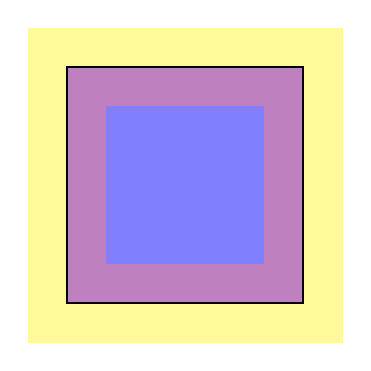
\begin{tikzpicture}[scale=1, transform shape]
	\node[minimum width=4cm,minimum height=4cm,fill=yellow!40]{};
	\node[minimum width=3cm,minimum height=3cm,fill=blue!50!red!50,draw=black,thick]{};
	\node[minimum width=2cm,minimum height=2cm,fill=blue!50!white]{};
\end{tikzpicture}
\end{center}
\end{figure}

	\end{column}
\end{columns}
\end{frame}

\begin{frame}[fragile]
	\frametitle{Block types and Position}
	\framesubtitle{Blocks, Inline-blocks \& Inline}

\begin{columns}
	\begin{column}{0.5\textwidth}
\begin{onlyenv}<1>
\begin{minted}{css}
li {
	display: block;
	text-align: center;
	padding: 5px;
}
\end{minted}
	
\end{onlyenv}
\begin{onlyenv}<2>
\begin{minted}{css}
li {
	display: inline-block;
	text-align: center;
	padding: 5px;
}
\end{minted}
	
\end{onlyenv}
\begin{onlyenv}<3>
\begin{minted}{css}
li {
	display: inline;
	text-align: center;
	padding: 5px;
}
\end{minted}
	
\end{onlyenv}
		
	\end{column}
	\begin{column}{0.5\textwidth}
		\begin{onlyenv}<1>
			\begin{figure}[h]
				\centering
				
\includegraphics[width=1\linewidth]{img/block.png}
			\end{figure}
		\end{onlyenv}

		\begin{onlyenv}<2>
			\begin{figure}[h]
				\centering
				
\includegraphics[width=1\linewidth]{img/inline-block.png}
			\end{figure}
		\end{onlyenv}

		\begin{onlyenv}<3>
			\begin{figure}[h]
				\centering
				
\includegraphics[width=1\linewidth]{img/inline.png}
			\end{figure}
		\end{onlyenv}

	\end{column}
\end{columns}

\end{frame}

\end{document}
